\documentclass[]{article}
\usepackage[pdftex]{graphicx}
\usepackage[top=1in, bottom=1in, right=1.25in, left=1.25in]{geometry}
\usepackage{hyperref}
\hypersetup{colorlinks=true, linkcolor=blue, urlcolor=blue}

\begin{document}
	\pagenumbering{roman}
	\tableofcontents
	\newpage
	\pagenumbering{arabic}
	\setcounter{page}{1}
	\thispagestyle{empty}
	
	
	\setlength{\parindent}{0pt}
	\setlength{\parskip}{6pt}
	
	% Eighth Entry
	\section{Optimizing O-O Python Code 02/20/2013}
		After optimizing the Python script for the analysis system, I decided to take the knowledge from creating that prototype to the O-O code I have been writing. The end goal of this work is to create a system that has comparable runtime to the Python script.
		
		\subsection{Script Optimizations}
			The big optimizations to the script were achieved by taking code that was being executed on every single cell and trying to perform the same action on an entire image so that each cell has less to do. After looking at my code, I did not really see any of these optimizations, but it was still taking 12 times as long as the script to run.
			
		\subsection{Profiling Code}
			I encapsulated my testing script into a single function so that I could run the Python profiler on the code. To do that, all I had to do was start an interactive Python shell, import profile and my testing file, and then execute ``profile.run(`test.main()', 'profiling-results')". The profiling made the code run even slower (I was testing on a 20 image set), but it ended up yielding valuable results. I then used pstats to reveal the method/function calls that used the most cumulative CPU time. For the 800 second run, the function used to convert the images to black and white used 500 seconds. 
			
		\subsection{Modification}
			The initial change I made was in the pImage class constructor where I set the self.im (the object representing the PIL image) from Image.open(filename) to Image.open(filename).convert("L"), which converts the image to black and white. I ran this and found that it took 60 seconds to run on 20 images, which is very close to the speed at which the script runs. 
			
		\subsection{Remaining Problems}
			Just like the script from a week ago, the O\-O code is leaving the images (now in B\&W) in memory for the entire run. On an 800 image set, the code will throw a too many files open error and if that is solved, it will throw a memory error. 
			
		\subsection{Solution to the File/Memory Problem}
			The solution seems to be fairly straight forward. I need to create a wrapper class for the PIL Image. Basically, it will hold a filename of an Image and provide the data when requested, but also allow for the data to be freed from memory when it is not being used. 
			
	% Seventh Entry
	\section{Python Memory Error 02/14/2013}
		Since the Python script can process images at a rate of approximately 5 seconds per image, it would take approximately an hour to process all the images for a class, which means that it meets spec. However, the script uses too much memory and causes Python to crash with an ``Out of memory" error. Colin and I sat down to try to fix this error so that we can have a working prototype for 700 images at tomorrow's panel. 
		
		\subsection{Why the error?}
			The problem is that we are trying to read 700 images into memory, which is too much and results in a Python Memory Error. The overall goal of this work session is to get the script to use a constant amount of memory regardless of the number of images. One of the big issues that we are facing is that PIL does not have a close() method for images because it uses lazy loading. This is nice because nothing gets loaded into memory until we need data, but it means that there is not a built-in way for us to say we are no longer interested in the data.
			
		\subsection{The cell\_image Problem}
			The script tried to create a huge array of cells (which is fine by itself because there is no image data being read into memory), but when the processing happens, the data gets pulled into memory and crashes the system. After an hour or so, we were able to tell the cropped data to live in a single cell so that we aren't keeping a huge cell array that has billions of bytes of image data. However, the memory was still increasing linearly with the number of images we were manipulating.
			
			As a bit of a relevant note, the ``del" keyword helps to free up memory. We found this out before trying to store just a single cell worth of data into memory at a time.
			
		\subsection{The im\_seq Problem}
			We are calling the crop method on images in an array of images to get the cell data. The cell data is freed every time we move onto another cell, but the problem is that the data has already been pulled into the im\_seq. Finally, we were able to get the program to read a single image into memory, perform operations on the data, and then release the memory that was being used. 
			
		\subsection{Benchmarking}
			Running the system on 20 images used approximately 150 MB of RAM on Colin's computer. Running it on a set of 200 images gave approximately 155 MB of RAM used. We are still running into problems with having too many files open when running on 700 images, but there is a post on Stackoverflow with a straightforward way of opening a file, creating an Image object, load the image data, perform operations on the data, release the memory, and close the file. 
	
	% Sixth Entry
	\section{Capture System App work 02/07/2013 - 02/10/2013}
		After capturing several sets of images, we found that the camera was automatically adjusting the brightness levels of the images when a professor walked in front of the board. This means that the luminance values for each of the cells in the image with the professor will be significantly greater than for the other images. As a result, the Python script classifies everything except for stroke cells as foreground cells.
		
		\subsection{Fixing the App Part I}
			My initial idea was that the white balance needed to be set to constant in the camera app. This was as simple as fetching the camera parameters, setting the white balance to incandescent (since it gave the best white color), and assigning the camera parameters back to the camera. Performing another capture revealed that this did not help with the brightness. Doing a bit of research into how to keep the brightness revealed that camera things such as ``aperture", ``shutter speed", and ``ISO" were the factors that would determine the brightness of an image. 
			
		\subsection{Fixing the App Part II}
			To confirm that I could keep the brightness of an image constant, I opened the Samsung camera app on the camera and set all the parameters to be constant. I then took two pictures; one of just a white surface and the other with my hand in front of the surface. With the ProPANE app, there was a visible change in brightness between the two images, but the camera app with constant settings gave the same brightness between the images. At first, this was promising because I would just have to make all the settings constant for the camera once the user pushed the ``Start Capture" button. 
			
			\subsubsection{Android Camera API}
				Looking through the official documentation for the Android Camera API, I came across a number of different parameters that controlled different aspects of the camera. However, reading through forums revealed that Android was never meant to control a physical camera and did not natively support the features I mentioned above.
				
			\subsubsection{Get Galaxy Camera Parameters}
				While looking for ways to set the ISO for a camera in Android, I read that there is a general way to set parameters using a (key, value) system for Android cameras. This allowed developers to add functionality to their cameras without altering the android OS. I was able to take the camera parameters object and convert it to a string, which revealed several hundred parameters that can be set for the Galaxy Camera. I started working my way through them looking for the parameters that set ISO, shutter speed, and aperture. Unfortunately, the advertised parameters list did not contain information about the three controls I was interested in.
				
			\subsubsection{Parameters Specified in the Kernel}
				Reading a forum about setting Galaxy Camera Parameters, I came across a post describing how there are non-advertised parameters that the built-in camera app must use to manipulate the controls for ISO, shutter speed, and aperture. Unfortunately, they are hidden in the kernel source code. Fortunately, the source code is available on Samsung's website. I combed through several thousand lines of the source code and found several parameters that are not advertised, but can be accessed (for example, there are several color effects that can be set, but are not advertised). 
				
		\subsection{Why Fix the App?}
			While trying to fix the app, I looked at the images that were the result of the Analysis System and I noticed that the stroke cells were being classified the same regardless of the white board brightness and I asked myself why do we need accuracy on the foregroud/board detection. The answer is that we do not. We are responsible for capturing the strokes and generating key images. If we detect everything in an image as foreground except for the stroke cells, it will require more image stitching to get the final key frame, but it is not a problem. This means that the analysis system can process images regardless of brightness. I have decided that the priority of the brightness level has decreased since it is not helping fulfill a specification and I have demonstrated that with enough time, I will be able to control the brightness. Also, chances are that those who frequent XDA developers will find the parameter soon and I can focus on other tasks such as converting the analysis system to C++ to decrease runtime, which is actually in the specification. 
			
		\subsection{Zoom Functionality}
			While setting up the capture system in a classroom, I started to worry that we would violate the 5 minute time limit for setting up the capture system since it had to be placed in a specific location to make sure that it captured only whiteboard. The obvious way to help with this was to add the zoom functionality so that the camera can be placed anywhere (preferably the back) in the classroom and use software to get rid of the board boundaries. While trying to ``fix" the camera app, I tested the zoom control I found out about in the advertised parameters. Adding two software buttons allowed me to zoom in and out on the board and should decrease the amount of setup time required and give us a bit more leeway when it comes to that requirement.
	

    	% Fifth Entry
    	\section{Setup Computer in BRKI 163 02/04/2013}
		Until this point, the entire group had been focused on different aspects of the image processing part of this assignment. Now that we have a working system (that still needs work), it was time to assign someone to work on the backend of the system that will handle the filesystem aspects of the backend system. Griffin was assigned with researching how to do the filesystem monitoring to determine when a new set of images is ready to be processed. Also, the system had not been tested on the linux system up until this point so it was time to start on that.

        	\subsection{Need to Change Tech Spec}
			Currently, the box in 163 is running 10.04 because that is one of the tech specs. While trying to install Samba and SSH, I found that this version of Ubuntu is not suppored by the packages and everything (GDM, Nautilus, ...) stopped working. I then installed Ubuntu 12.04 (LTS) on the box and was able to install Samba and OpenSSH-Server without any problems. Looking at tech spec 5.1.1, I would like to change the requirement from 10.04 to 12.04. The rationale for using 10.04 in the tech spec document is: ``This requirement exists to ensure that the software can be run on a free-of-cost operating system''. Since 12.04 is also a free-of-cost operating system, there is no real reason not to change the spec. Also, the Python analysis system was tested on a 10.04 virtual machine and ran successfully so the analysis system meets the spec and it is only the extra feature to make the end user's life easier that will not work on 10.04. I will send out an email to the clients with a formal requirement change request. 

       	 \subsection{Server Configuration}
			After installing 12.04, I installed Samba and configured it so that there is a share in the /home/propane/ProPANE directory where images will be placed for processing. The server is accessible through the URL propane.stahlfeld.com (this was the easiest/fastest way to get things set up for our testbed). Eventually, we hope to get something like propane.bucknell.edu. I was able to access this share through external linux and windows boxes. I also setup the OpenSSH-Server so that we should be able to test things without having to go to the lab.

       	 \subsection{Testing Analysis System}
			I installed git and cloned the ProPANE repository into my home directory on the linux box and tried to run the system. I got an error saying that the numpy module could not be installed. To install numpy, I had to install pip using apt and then use pip to install numpy. Once numpy was installed, I ran the system successfully on a set of 6 images. It took just over 200 seconds to run, which would give a runtime of approximately 6 hours for a full set of 600 images. This was expected since the clock speed of the linux box is 1.86 GHz compared with my laptop's 2.4 GHz (both processors are Core 2 Duos). 6 hours is still well within spec.

    % Fourth Entry
    \section{Python Optimization 01/31/2013}
	Comparing the script runtime to the O-O code runtime made me believe that I was doing something wrong in one of the objects and that was the reason for the excessively long runtime. I decided to compare the number of different calls from the script to the O-O system. 

		\subsection{Comparison of Calls}
			The initial comparison revealed that the script did not make calls to anything except for modules in the PIL libraries and the numpy library. These were the same calls that the O-O system used so it could not be the actual calls themselves. I then started comparing the number of calls. There were the same number of calls to perform the math on the cells (generate histogram, adding histograms, getting luminance values...). Finally, I saw that the script calls the Image.open(JPEG FILENAME) once per image. Looking at the O-O program, the Image.open(JPEG FILENAME) gets called everytime a cell needs to access the data so it would be L * W * N where L is the number of cells per column, W is the number of cells per row, and N is the number of images.

		\subsection{Speeding Up the Code}
			The O-O code calls the Image.open method so many times because I wanted to be able to test the pCell class before writing the pImage and pImageSequence class. Now that everything seems to be working (and it is just slow), I can go back and change this to be smarter. To fix this problem, I changed the constructor for the pCell to take an open PIL file descriptor instead of a filename. This way, there will only be N open calls and the image descriptor will be shared between all pCells of a pImage. Note that this should not dramatically increase the memory footprint of the system because the open call does not load image data into memory, the data is loaded when something makes a call that requires data (e.g. crop()). 

      		\subsection{Performance Results}
			Looking at the code, I made the claim that we could expect O(N) runtime where N is the number of images that have to be analyzed. Running the system on a 6 image set gave a runtime of 182 seconds. I then made the statemnt that it should take approximately 30 seconds to process a single image. Running the system on a set of a single image gave a runtime of 29.5 seconds. This showed that my claim about the system runtime was correct and that we should expect approximately 5 hours to process a 600 image image set (a full class). This is well within the specs, which state that we need to have a turnaround time of 24 hours. 
            
	
	% Third Entry
	\section{More Implementation 01/28/2013}
		
		\subsection{pImageSequence Completion}
			The pImageSequence class can be given a directory containing JPG images and it will generate pImages out of those images and classify the cells. I have only been running the tests on two identical images. This test was designed to show that the class can handle multiple files without crashing. This test by no means tests the image processing functionality of the program.
			
		\subsection{Testing}
			Since we already have a script that has produced acceptable results on a set of images, I had a good way to compare the images generated by the O-O code. After running the code on the same set of images, it was clear that the process was taking extremely long compared to the script. Assuming an O(n) runtime where n is the number of images, the process would take nearly 50 hours to run on a 600 image set (approximately the same size as what will be expected from a normal class). This is by far the largest problem we have encountered so far because it means that this implementation will not meet spec since one of the specs is that we need to process the images in 24 hours. 
			
		\subsection{Options for Speedup}
			Bottom line: Python is slow. We have been using it because it is extremely easy to prototype in (see work completed thus far). However, it may not meet the performance requirements. Below are some of the options that have been considered thus far to speed things up.
			
			\subsubsection{SciPython, Cython, NumPy, etc}
				Performing a quick Google search shows that there are a number of tools available for speeding up Python code by using special modules such as the ones listed in the title of this section. The modules will help by making the underlying python structures resemble the C structures more. 
				
				Cython claims to be able to give up to a 35\% speedup by just using its compiler on the Python code that has already been written. However, this is the best case scenario. It also provides significant speedup by statically typing the variables used in Python code. This would be helpful for some of the math intensive methods such as adding thousands of histograms or calculating the stddev and mean of cell data. This seems like a good starting point if we decide to use Cython because it will show significant results without changing much.
				
			\subsubsection{Switching to a Different Language}
				Switching to C/C++ seems like an obvious choice because both languages are extremely fast. The downside is that they are not as easy to use and the parallelism for development would decrease because Griffin and Colin are lacking in their knowledge of C/C++ as it relates to this project. Furthermore, Python is extremely good for the backend daemon that needs to monitor the file system so it would make integration harder if we had to use Python for the backend daemon and then C/C++ for the analysis system. On the plus side, the pCell maps extremely well to a C struct (great for speed). Using C++ for this project would be relatively trivial (although lengthy) because with Python, we already have the classes implemented and can essentially just convert them into C++ syntax. We have shown that the implementation works, it just needs to be tweaked. 
			
			\subsubsection{Optimize the Python Code}
				Taking a step back, we have a script that can process the 6 images in approximately 60 seconds. By making this code O-O it takes 1316 seconds. While Python is known to be slow, it was capable of processing the images in 60 seconds and there is no way that taking that code and making the most streamlined objects could possibly result in a 20x slowdown. I am convinced that there is something in the code I wrote that is not behaving as I expected. Before switching languages or anything like that, I want to try to find all of the places where the code can be optimized for speed. 
	
	% Second Entry
	\section{Implementing O-O Analysis System 01/24/2013}
	
		\subsection{pCell}
			Started work by implementing the pCell class, which frames the data in an individual cell of the image. Note that it does not contain the actual data of the image (this should help reduce the memory footprint). Each pCell will have a method called classify() that will allow the pCell to classify itself as a board, stroke, or foreground cell. This classification will be used in later processing for image stitching and further refinement in the classification of other cells.
			
			After talking to Colin about this method, each pCell will need to know the color of the whiteboard area that it frames. This involves calculating the most common luminance value for the cell over time (i.e. multiple images). This calculation will have to happen at the ImageSequence level of the class structure so I am just leaving it as an instance variable for use later.
			
		\subsection{pImage}
			This class is essentially a way of organizing pCells. It does not perform any calculations on the data in the cells to determine their classification. This does not mean that it can be replaced with a 2D list because more functionality will be required for the image stitching process and for debugging (allowing cells to be enhanced to show visually how everything works).
			
		\subsection{Things to Remember for Next Time}
			The pImage and pCell class are working with the exception of the pCell classify() method. This was left out because Colin was the one working on the math for the image processing and he should be the one to put that math into the pCell class. The pImageSequence class needs to be created and gather histograms for all of the cells in all of the images. 
	
	
	% First Entry
	\section{Object Orienting Python Code 01/21/2013}
		The ProPANE system can be broken down into three software components: the capture app, the analysis system, and the backend manager. The capture app produces a folder containing images of a white board. The analysis system takes the images and generates key images. The backend manager is the interface between the user and the analysis system.
		
		\subsection{Backend Design}
			The idea for the backend is to have a user connect to a Samba share on the linux computer and drop the folder containing their images into a dropbox type folder. The backend daemon will be monitoring this directory for changes and when it notices the new images, it will move them to the final location and start an instance of the analysis system.
			
		\subsection{Analysis System}
			The analysis system will process the images to generate the key frames and notify the backend daemon that it is complete. The entire image set will be stored in a directory structure as follows.
			
			\begin{itemize}
				\item CaptureSet1
					\subitem{EntireSet}
					\subitem{KeyFrames}
			\end{itemize}
			
			Where CaptureSet1 refers to a class period capture sequence, EntireSet contains the all of the images taken during the class, and KeyFrames contains the images generated by the analysis system.
			
		
	
	% Twenty Fourth Entry
	\section{Panel 3 Preparation 11/28/2012}
	
		Tonight's work consisted of generating the Powerpoint that can be accessed on the ProPANE website. We tried to minimize the amount of text that went on the slides so that people would focus on what we were saying rather than trying to read everything on the slides. The major items we wanted to convey in the PowerPoint were:
		\begin{itemize}
			\item Camera selection
			\item Tripod selection
			\item Analysis system design
			\item Capture system design
		\end{itemize}
	
	
	% Twenty Third Entry
	\section{Work on Design Report 11/19/2012}
		
		\subsection{What goes in the design report?}
			Obviously, some of the major decisions made by the team have to be included in the design report, but the minor ones do not belong in it (they belong in the worklog). The decisions that need to be addressed in the document ares as follows:
			\begin{itemize}
				\item Camera selection
				\item Tripod selection
				\item PIL selection
			\end{itemize}
			
			
		\subsection{Layout of Android app}
			While looking at the technical specifications and considering what the clients would need, I decided that the Android app would need at least one extra screen (in addition to the Start Capture screen). Since professors will want to capture images from different classes, they will want to have the images in some sort of organizational structure so that they can be sent to the analysis system easily. I want to include a screen that will let the professor select a name for the directory where they want to store the images. The addition of this screen will only mean the addition of one more activity and then the second activity will have to retrieve the results of the form in the original activity. This is the same principle as the HelloWorld program written about in a previous work log so it will not add complexity to our design. This could be considered as scope creep since it was not included in the technical specification. However, writing the HelloWorld also was not in the technical specifications, but it had to be done and made my life easier. Adding this other screen should help with testing so for these reasons, I am deeming it necessary.
	
	
	% Twenty Second Entry
	\section{Cleanup of Android app Code 11/15/2012}
		
		\subsection{Making code more readable}
			Looking through the app I wrote, I realized that it was impossible to read and had several methods, instance variables, and objects that were never used, but looked like they could be used. This seems natural since it was my first attempt with Android. I went through the code and removed all of the unused pieces and added comments so that it is easy to follow. While doing this, I thought of a potential problem addressed in the next section.
			
		\subsection{Stack overflow problems}
			At first, I though that the PictureCallback object would keep pushing new (recursive) stack frames since the takePicture method seems to call itself again through the use of the PictureCallback. Thinking about it in a bit more detail, this should not actually be a problem. The takePicture call will finish in the PictureCallback and since it returns, the stack frame will be removed. Once the image data arrives to the PictureCallback, it will save the data and call the takePicture method again (theoretically in the same place on the stack as the previous call). By using the PictureCallback, we avoid the problems of ``recursively" calling the takePicture method. 
	
	% Twenty First Entry
	\section{Implementation of postDelayed() in Android app 11/13/2012}
		Altered the Android app so that when the Start Capture button is pressed, the app will start to collet images at the a standard rate.
		
		\subsection{startCapture() Implementation}
			StackOvelflow said not to delay the GUI thread in button callbacks for very long, so I removed the loop and Thread.sleep() lines. The startCapture() method just creates a new PictureCallback that then gets used to take a picture.
			
		\subsection{PictureCallback Implementation}
			The PictureCallback is the place where the actual looping takes place. It saves the returned JPEG data as a file and then calls the takePicture() method with itself as the PictureCallback. To make sure that this does not try to loop infinitely fast, I used the PostDelayed that waits 5000 milliseconds and then calls the takePicture method. 
	
	% Twentienth Entry
	\section{Android Power Management 11/09/2012}
		
		\subsection{Galaxy Camera Battery}
			After reading an article on the Galaxy Camera, I found that the battery should be sufficient for a single class, but it might not be good enough for a professor who has a full day of teaching classes (or just one long class). According to the article, the main use of the battery was the LCD screen since it is so large and bright. We should be able to have the app turn the screen off when it is capturing so that it does not waste battery (and does not distract students in class. 
			
		\subsection{Android Services}
			According to the Android developers website, the capturing activity can start a Service that will run in the background and continue running even when the screen is off. Using a Service, I should be able to alter the ProPANE app so that it does not waste the battery by unnecessarily using the LCD screen. 
	
	% Ninteenth Entry
	\section{Loop takePicture() in Android 11/06/2012}
		The goal of this work is to extend the capabilities of the Android app to take multiple pictures with a 5 second delay in between each picture.
		
		\subsection{Simple for Loop}
			My initial attempt at this was to put the code that performs the picture taking in a for loop and call Thread.sleep(5000). Testing this out gave unexpected behavior. The app appears to be taking pictures every 5 seconds (i.e. the preview of what the camera sees pauses for about half a second every five seconds), but checking the output folders shows that one or sometimes two pictures get taken instead of the five or six that that the loop specifies. 
			
		\subsection{Online Research}
			Googling the problem has yielded two pieces of information that appear to be useful. I came across code that is the same for loop that I am using, but does not have a delay at all. The problem with this code is that the next takePicture() is being called when the first one is still taking a picture. The solution is to tell the PictureCallback to call the takePicture(). This ensures that the camera is not busy during the second call, but it means that the number of pictures being taken will have to be kept track of by means of an instance variable instead of a for loop. 
			
			The other piece of information that is useful is the postDelayed() method because it seems to do the waiting that is desired. An example of it can be found on StackOverflow \href{http://stackoverflow.com/questions/4111905/how-do-you-have-the-code-pause-for-a-couple-of-seconds-in-android}{here} and the API can be found \href{http://developer.android.com/reference/android/os/Handler.html#postDelayed\%28java.lang.Runnable,\%20long\%29}{here}.
			
		\subsection{Future Work}
			I am going to try to use the above two pieces of information to have the app take a picture on a button press, then the PictureCallBack will use the postDelayed() method to take another picture until the app is killed. Eventually, there will have to be a way to stop the app from taking pictures without killing it. My thoughts on that right now are to include a stop button that will change the state of an instance variable that the PicutreCallBack will examine and not call takePicture() anymore.
		
	
	%Eighteenth Entry
	\section{Successful Android Camer App 11/01/2012}
		I was able to get an app running on my phone that would let me push one button from inside the app and it would take a picture. It displays a preview of what the camera sees and saves a picture to the internal SD card. 
		
		\subsection{Solution from Previous Attempts}
			After scouring the camera API, I found that a camera needs to be passed a frame where it can show the preview before the camera can take a picture. I followed the tutorial from before, but this time included the part about creating a preview and was able to get the system to function correctly. The code is available on  GitHub under the Code/Demos/Android/CameraTest (on the CameraTest\_1.0 branch). 
			
		\subsection{Future work}
			The future work on this part of the project will have to make the system take multiple pictures on the push of the start button. This SHOULD just putting the take picture in a for loop and waiting a specified amount of time. 
			
	
	% Seventeenth Entry
	\section{Consideration for Construction of Analysis System 10/31/2012}
		The best way to implement a project of this size that is maintainable is to use object oriented design. I think this project lends itself well to object oriented design. After talking to Colin and reading his work log, it is clear that he has the ability to write a Python script that can break a JPEG into cells and manipulate those cells. While he is working on the image processing to get the cells normalized, I think it is my responsibility to make sure we have a rough design of how the work we are doing will fit together next semester. \\
		\\
		Right now, I see that there will be at least three classes. At the top level, there will be a sequence of images where methods should be available to find key frames, do image stitching, and the other high level tasks. The next level down will be a single image where methods should be available to normalize the JPEGs, retrieve information about different regions of the board, and other single image tasks. The lowest level down will be a cell where methods should be available to do pixel by pixel by pixel manipulation, retrieve values from the overall cell, and any other pixel related tasks. 
		
		 \subsection{Image Sequence}
			Every lecture (each time the capture system is started and stopped) should map to exactly one image sequence that will be composed of numerous images. The purpose of this class is to use the information from the image objects to create the final key frames. The image sequence will keep track of the amount of information on the board based on time. The image sequence will use this information to construct key images by stitching images together to remove the professor from the image with the most information on it. 
			
		\subsection{Image}
			This is class provides a means for the image sequence to manipulate the actual images. For example, the big one for stitching is cutting a cell from one image and pasting it into another image. My idea is to represent the captured JPEG data as cells in a 2 dimensional array like structure so that cells can be pulled from and pasted into images with just an (x,y) coordinate pair. This class will also have to collect the information needed from the individual cells.
			
		\subsection{Cell}
			This should be the only class that has direct interaction with pixels of an image. This class will require methods for finding the data required by the algorithms in the Microsoft WCS such as: maximum pixel value (for finding whites).
		 
	
	
	% Sixteenth Entry
	\section{Configuration of Development Environment 10/27/2012}
	
		\subsection{OpenCV Python Background Detection}
			While waiting for Ubuntu to download, I came across \href{http://opencvpython.blogspot.com/}{this} article about background detection using OpenCV and python. It looks like this article provides another way of removing a professor from images by detecting what is background and what is not. Based on my initial reading, it looks like it takes a weighted average of a sequence of images. For situations where traffic is supposed to be removed from the background, it works incredibly well, but I am a bit unsure as to whether it will work for when a professor is in front of the board for extended periods of time without moving. It seems like the "residual" professor coloration would alter the color of the whiteboard in the image. It is possible that we could perform a the weighted average on the images and do the filtering later, but this would not follow the process in the Microsoft WCS paper. 
	
	
	
	% Fifteenth Entry
	\section{Post-Panel 2 Reflection and Memo Creation 10/25/2012}
		The big thing on my mind is how the image processing is going to work. There are more unknowns regarding the image processing than any other area of the project. Right now as a group, we do not really know enough about image processing to even know what we should be looking at software wise. I found \href{http://en.wikibooks.org/wiki/MATLAB_Programming/Image_Processing_Toolbox}{this} online book that should help with learning about what we will have to do. Although everything in it is written in MATLAB, we should be able to take the concepts away and apply them to the language that we choose. 
		
		
		\subsection{More on WCS}
			The Microsoft WCS paper is basically the starting point for all of the research that is being done right now. It contains the algorithms used by the team to perform most of their image processing. Most of it seems to be about collecting information on all of the pixels in an image and using that information to alter each pixel for a desired result. This process screams to use Python because of the flexibilities of the builtin list data structure. Although the language is slow, it provides some of the same features as the vectors/arrays in MATLAB. 
			
		\subsection{ImageMagick}
			In Panel 2, a colleague recommended the ImageMagick package since it has bindings for most of the popular languages (see list \href{http://www.imagemagick.org/script/api.php}{here}). The problems right now are that I cannot get it installed on my Mac (time to set up the Linux box) and there is essentially no documentation. Even if I could get it installed, I cannot find any documentation on how to use it in Python or Java.
			
		\subsection{OpenCV}
			OpenCV keeps popping up during my research into image processing services, but I did not look more into it because it is such a large package and my lack of knowledge about the field made learning about the package very prohibitive. The plus side to this is that it has enormous amounts of documentation. The only problem is that I need to learn more about the actual image processing. 
			
		\subsection{Overall Image Processing Thoughts}
			I do not think that we need a massive piece of image processing software that essentially has a command line for Adobe Photoshop. The design of the system right now is to break the image into cells and deal with each cell. This sounds like OO programming. Create a class that represents a cell and a class that represents a collection of cells (i.e. an image). Since PIL, OpenCV, and ImageMagick all seem to be able to split images into cells and gather image information into list/array data structures, it does not seem to matter which service we use. 
			
			The biggest risk area that we know of is the image stitching, but I think it should be fairly straightforward (notice: not easy) since we will be using a cell based approach. My thoughts on this part of the project are as follows: 
			\begin{enumerate}
				\item Find key image based on number of ``mostly white" cells
				\item Identify ``foreground" cells
				\item Replace each "foreground" cell with the most recent version of the cell that is not foreground
			\end{enumerate}
			The immediate problem I see with this is if a only a small portion of the cell is foreground and the rest is information. The next most recent cell may not have all of the information in it and the key image would not have all of the information (BAD). I think the solution to this is to make the cells as small as practical. This way, if the above scenario happens, we would only be losing part of a letter instead of possibly a whole word. 
		
		
		
	
	
	% Fourteenth Entry
	\section{Examination of Android Development 10/23/2012}
		Since we are planning on using an Android based capture system, it seemed logical to start looking at how apps are developed. I wanted to create a simple camera app as a demonstration that it can be done so I started working on \href{http://developer.android.com/guide/topics/media/camera.html}{this tutorial}.
			
			\subsection{Camera App}
				Based on the number of Google hits for ``android camera tutorial", I figured it would be fairly simple to tell the camera to take a picture and store it somewhere. It looks like there are two ways to take a picture. One is to use an intent to request that another application take the picture. I tried this code, but it just opens the camera app, which does not help the project at all.
				
				The other solution looks to be more along the lines of what we need because it essentially creates a camera application that can be controlled directly. I do not know enough about Android at the moment to be able to understand what all the code fragments do and where they need to be located within the app. It is time to start learning how Android works.
				
			\subsection{Learning Android}
				I followed the first tutorial on the Android developers guide mentioned above and have learned several pieces of useful information.
				
				\subsubsection{Callback Functions}
					There is no need to define button listeners. Specify a callback method in the XML document. 
					
				\subsubsection{Activities/Intents}
					Every screen that gets shown in Android is called an Activity. It looks like intents can bind two activities together. For right now, all that means to me is that I can start another Activity using an Intent, which allows me to show a different screen to the user.
					
				\subsubsection{Passing Information}
					Information can be passed from one Activity to another using the Intent.putExtra method, which pairs a key with a value and passes the pair to the receiver of the Intent.
	
	
	
	% Thirteenth Entry
	\section{Examination of PIL 10/19/2012}
		The Python Imaging Library (PIL)  provides a module for Python for image processing. Colin came across this module and asked me to take a look at the features. To test out some of the features, I downloaded an image (see below) of a whiteboard and ran it through several filters to generate the following images. I am using the Enthought distribution of Python 2.7 and PIL came installed by default.
	
		
		\subsection{How it is done}
			The following code shows how an image can be imported, run through a filter, shown, and then saved.
			
			\begin{verbatim}
			from PIL import Image
			from PIL import ImageFilter
			
			image = Image.open("original.jpg")
			new = image.filter(ImageFilter.FIND_EDGES)
			new.show()
			new.save("find_edges.jpg", "JPEG")
			
			\end{verbatim}
			
			Note the simplicity of this program. Looking at some of the code to perform the same operation in Java reveals that Java is a much more verbose language when it comes to the basics of image processing.
		
		\subsection{Generate Images}
			All of the images generated during this examination are stored in the "images/python-filters" directory under the Stahlfeld\_Worklog source directory. It is hard to see differences in some of the images in this document.
		
			Running the "image.size[0]" gives the width of the image and "image.size[1]" gives the height of the image.
			
			The following is the downloaded image from Google Images.
			
			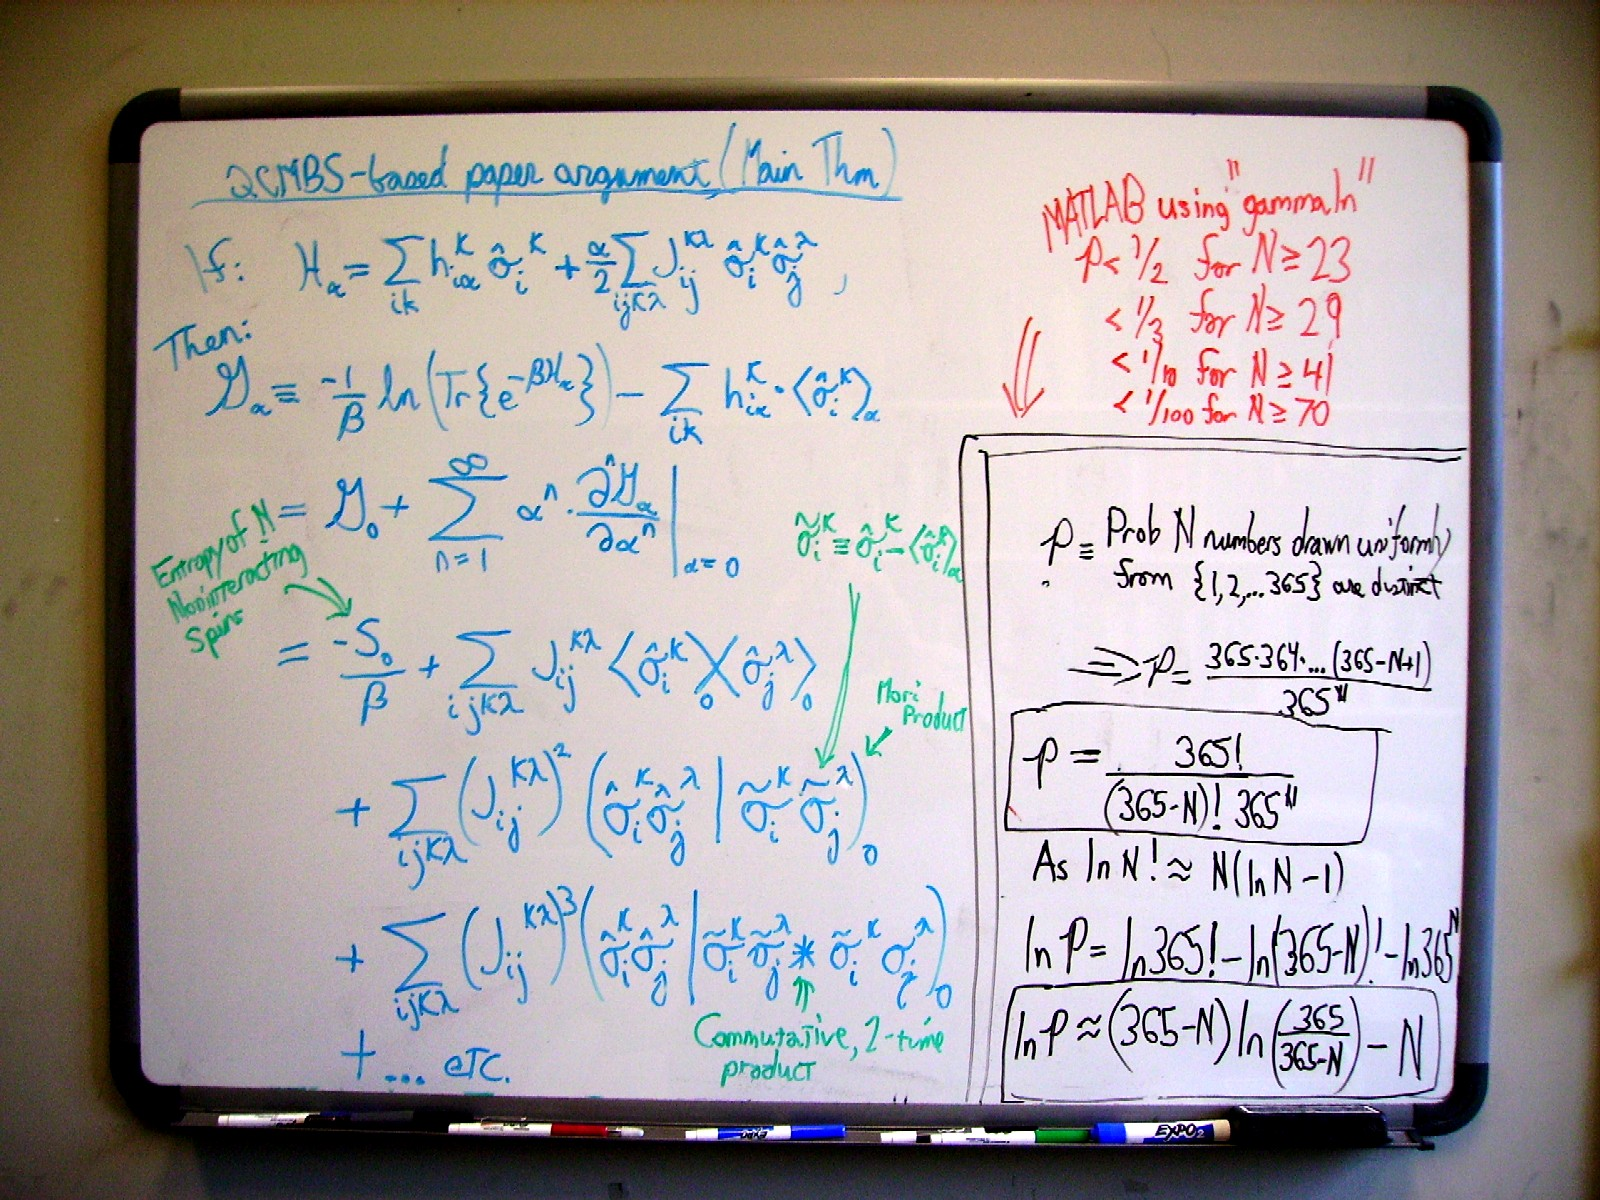
\includegraphics{images/python-filters/original.jpg}
			
			The following are filters of the different image. Note that all of the filters are built-in and can be found \href{http://www.pythonware.com/library/pil/handbook/imagefilter.htm}{here}.
			
			Below is the FIND\_EDGES filter
			
			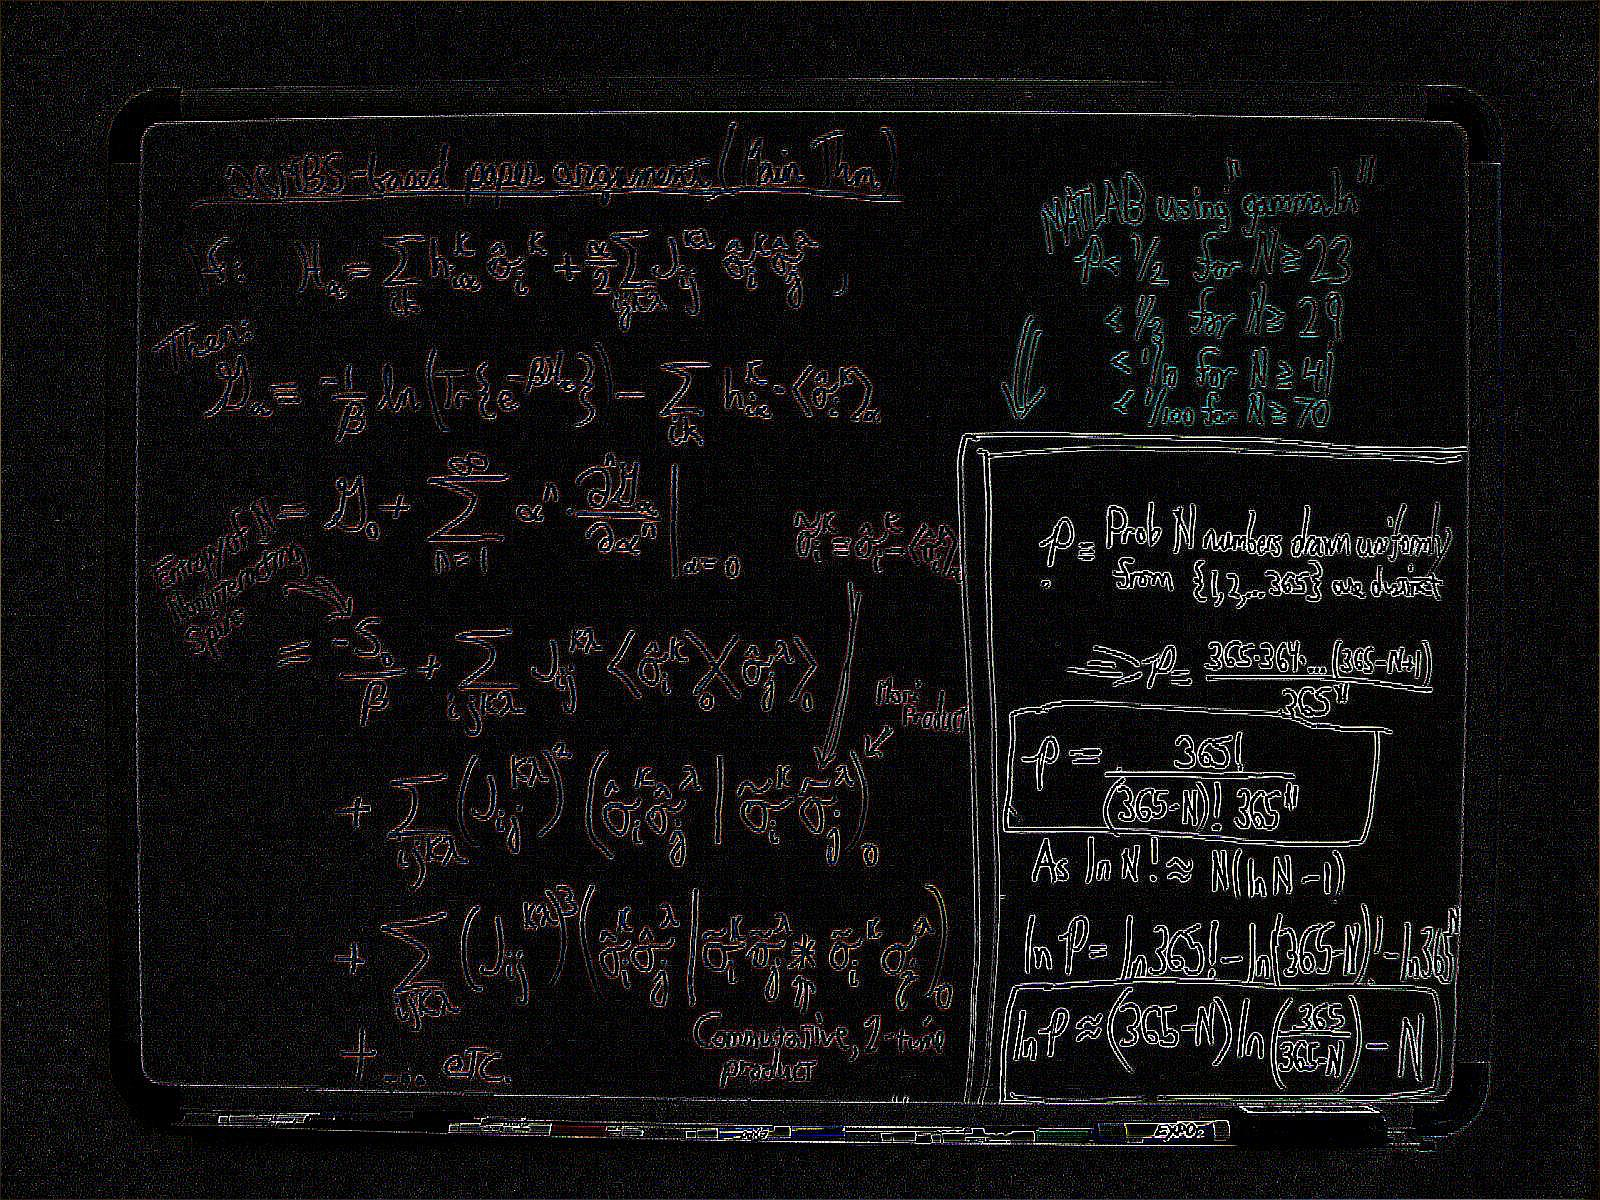
\includegraphics[scale=0.238]{images/python-filters/find-edges.jpg}
			
			Below is the EDGE\_ENHANCE\_MORE filter
			
			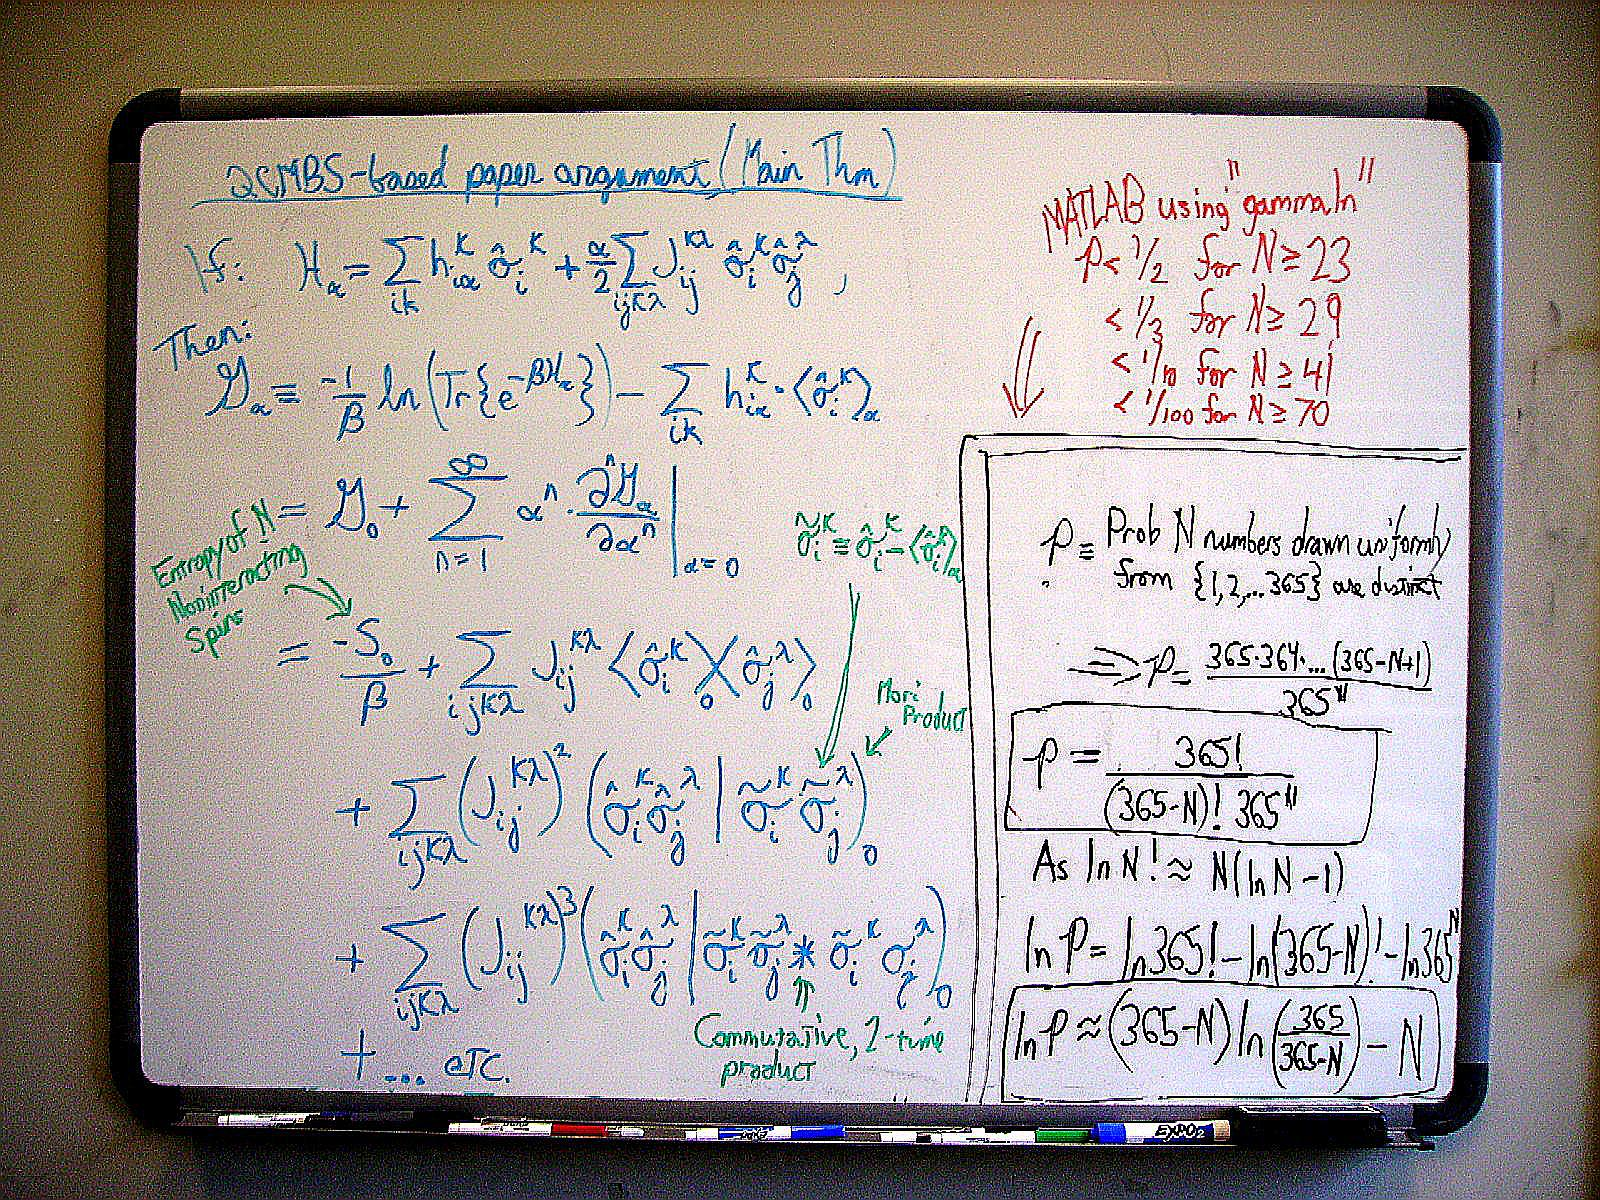
\includegraphics[scale=0.238]{images/python-filters/edge_enhance_more.jpg}
		
			Below is the DETAIL filter
			
			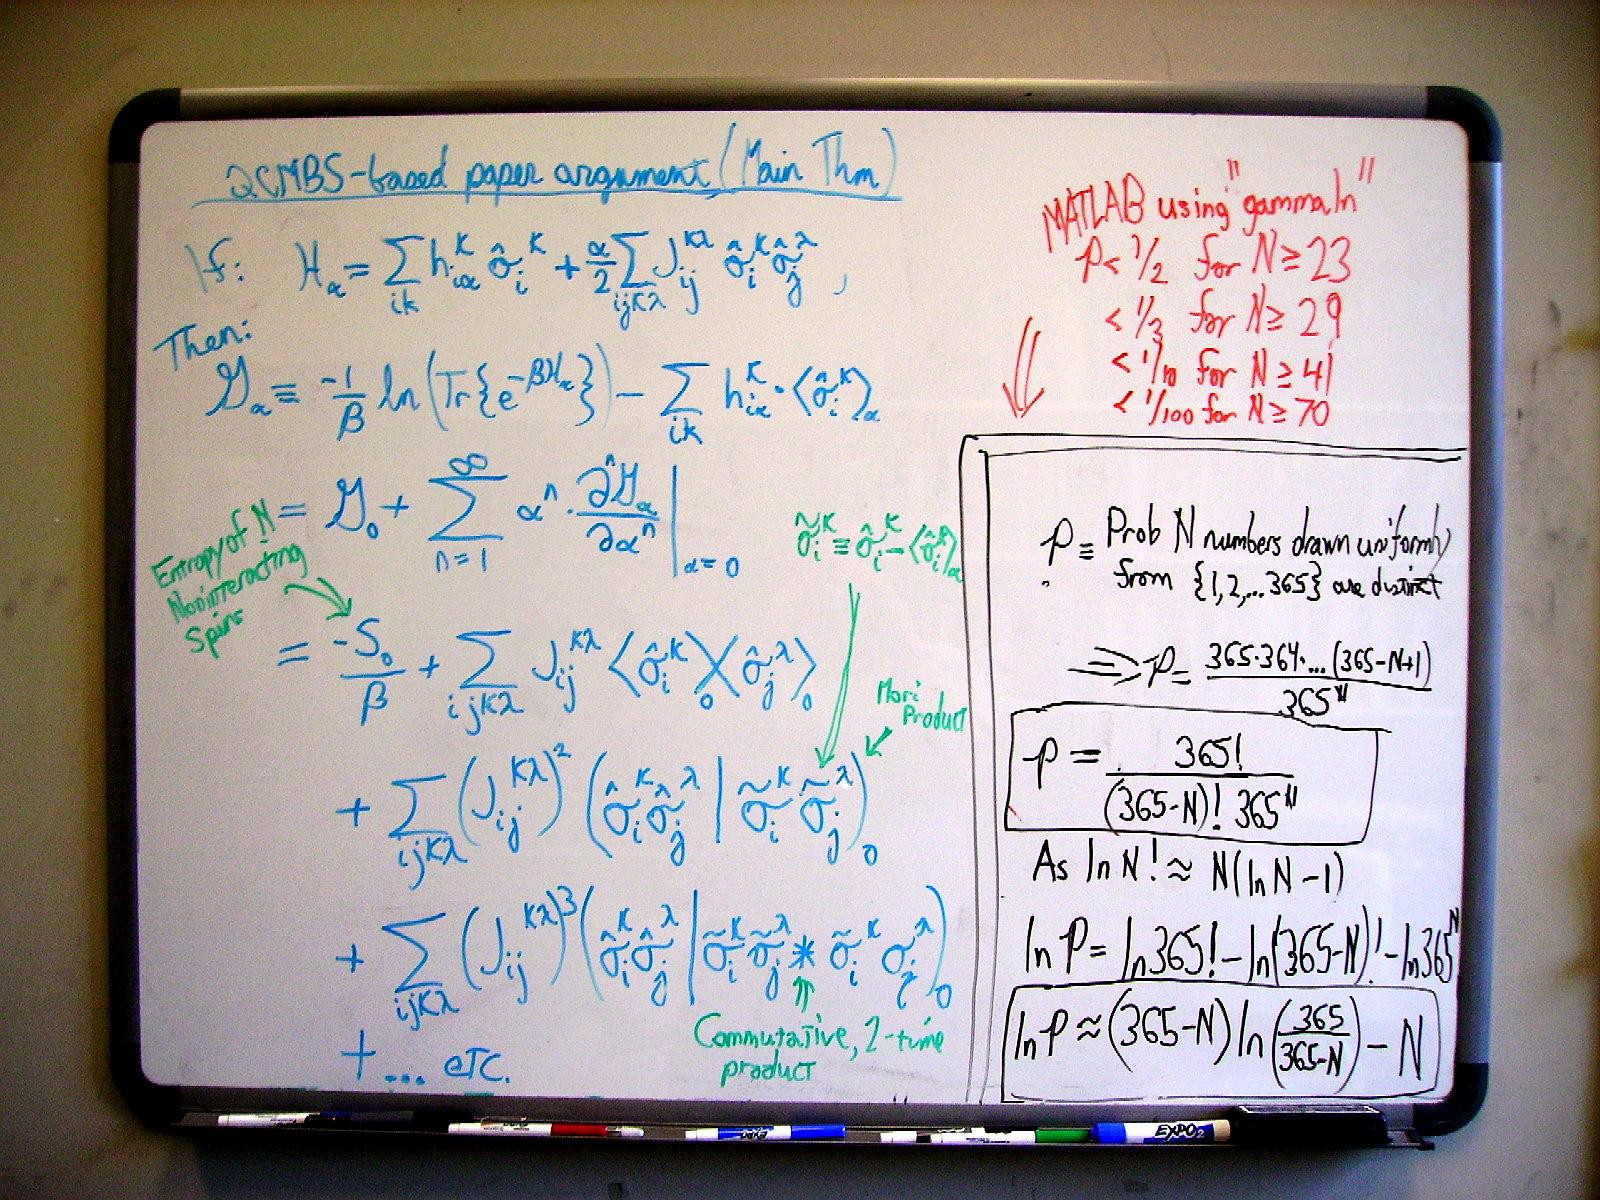
\includegraphics[scale=0.238]{images/python-filters/detail.jpg}
		
	
	% Twelfth Entry
	\section{Start Dividing Up Individual Tasks 10/18/2012}
		Starting to list out all of the tasks that must be accomplished by the end of the semester. Group them based on who is responsible for completing each task. This provides a certain amount of accountability for each part of the project. The tasks have been divided so that there is some evidence that the task was accomplished. Hopefully, the results of these tasks will demonstrate that the project is ready to enter the design phase. Each task is a proof-of-concept to demonstrate that we can accomplish the larger goals of the project.
		
		\subsection{Group}
			\begin{itemize}
				\item Gantt chart (probably using the following sections)
				\item Specification for deliverables
				\item Develop resources document
			\end{itemize}
	
		\subsection{Colin}
			\begin{itemize}
				\item Contact Microsoft about WCS
				\item Divide image into cells using Python
			\end{itemize}
		
		
		\subsection{Griffin}
			\begin{itemize}
				\item Collect images of whiteboards using various cameras
				\item Examine "CamScanner" app source code to find anything possibly relevant
				\item Determine settings required for capturing whiteboard information
			\end{itemize}
		
		\subsection{Phil}
			\begin{itemize}
				\item Access camera on Android based device
				\item Determine Java appropriateness for image processing
					\subitem{If appropriate, divide image into cells using Java}
				\item Classify cells as "white", "mostly white", or "colored".
			\end{itemize}
	
	
	% Eleventh Entry
	\section{Adding Meeting Minutes and Additional Features 10/12/2012}
		
		\subsection{Re-format Site}
			When adding the minutes to the website, the file browser started to look cluttered so the layout of the site was changed to be a list where each entry represents a meeting. Each meeting has a name, a minutes file, an agenda file, and the date the meeting occurred on. This system appears to organize the site as well as allows for storage of files on github via a hyperlink. The reasoning behind this is to not use up the quota on the Google site, which is limited. By making an open project on github, the project is guaranteed unlimited space. 
			
		\subsection{Finishing Touches on Tech Specs}
			After reviewing the feedback from meetings, I realized that I needed to add a comment about how resolution will not be a problem for the project since the Microsoft paper used a 4MP camera 10 years ago and it was not a problem.
		
	% Tenth Entry
	\section{Finishing Technical Specifications 10/11/2012}
		To make sure that the work done in this worklog appears on time on the ProPANE website, I have removed the file from the site and replaced it with the link to the worklog on github. This will insure that on every push the worklog gets updated on the site. Have successfully tested this method and it works.\\
		
		\subsection{Note on Git Usage}
			Forgot to pull down before editing and git gave a message like:\\
			\includegraphics[scale=0.5]{images/git-problem1.jpeg}\\
			To fix this, I added the top and bottom tex files listed in the modified list. Committing again resulted in an error free commit.\\
			Need to remember to pull before editing. 
			
		\subsection{Addition of Priorities}
			Prioritized the technical specifications based on the following qualifications. The priority is HIGH if a violation of the specification would result in a non-functional system. The priority is MEDIUM if a violation of the specification would result in a functional, but non-usable system. The priority is LOW if a violation of the specification would result in a functional usable, but difficult to use system. \\
			\\
			A HIGH priority spec is essentially a 'mission critical' specification. Violation of a MEDIUM priority spec essentially says that the system is capturing and analyzing the images, but it is violating the portability requirement for the system. Violation of a LOW priority spec basically says that the system is functional and portable, but will require extra resources (time, software, etc) to use.
			
	% Ninth Entry
	\section{Group Meeting for PSM 1 10/01/2012}
		The main issues discussed were the resolution issue and the interface issue that were brought up during the initial panel. The resolution issue was basically the agreement with the clients that there will have to be a certain number of pixels given to a certain portion of the board. The interface issue is that not all professors would feel comfortable using Linux for the analysis system. 
		
		\subsection{Resolution Issue}
			This does not seem like it will be an issue because the Microsoft paper shows that the goals we wish to accomplish were accomplished using a 4 MP camera from 10 years ago. Given that the setup for data collection in the paper is nearly the same as what we are using, the progression in camera technology should not be a problem.\\
			\\
			However, this IS an issue because it is an area that could possibly pose legal problems. If the resolution is too poor, then the system would be giving ProPANE reliant students a disadvantage. In my opinion, that would be a complete failure of the project.
			
		\subsection{Interface Issue}
			This issue could pose a problem for the project and will have to be investigated. Given that professors do not want to interact with any of the Linux GUIs (and there is no reason why they should). We will have to find a way to browse/export (key) images through a classic interface (i.e. OS X, Windows 7, Windows Vista). The three options I see for solving this problem are: creating our own GUI, give path names, or make a separate directory. 
			
			\subsubsection{ProPANE GUI}
				Creating a GUI would be an extra step in the project and it seems like it would fall under the category of scope creep (let's save this for version 2, but make initial notes on what it will have to do).\\
				\\
				The GUI would have to be cross platform and not require anything special (make it accessible to everyone). To me this sounds like a website. Given my website skills (PHP, Ruby on Rails, MySQL, AJAX etc), this seems like the best way to go. Everyone is comfortable using a browser so it would relatively simple to create the GUI.
				
			\subsubsection{Path Names}
				Theoretically the analysis system would generate key images and know the path to the key images. If everything is kept in an SMB share (where security will already be taken care of), users would be presented clickable links to the key images that would be on the share. This would require an image browser/editor on the client computer, but relatively little work for the group.
				
			\subsubsection{Separate Directory}
				Basically, this would have the analysis system have a directory titled ``All\_Images" and one titled ``Key\_Images". This would make life incredibly easy because a key image would just have to be copied from all images to key images. However, the drawback is that since the key images will not be living near images taken at around the same time. If the key image is wrong, the professor would have to go back to all images and search for the key image and then find the the correct key image. The above system would allow for this with just an arrow key action. 
	
	% Eigth Entry
	\section{Review of Panel 1 Notes 09/28/2012}
		
		\subsection{Tech Specs}
			Judging by the reactions of the panel members, the technical specifications are coming along well. The idea of the analysis system being run on a Linux platform brought up a problem that some professors will not be comfortable using Linux and would prefer OS X or Windows. It seems like a good idea to keep the actual analysis on Linux (keep it open!), but there will have to be an easy to access interface for browsing images. The first thing that came to mind was a web interface. A web interface would be a good idea because it is platform independent and it makes GUI programming a lot easier than using something like QT. It might also allow for integration with Moodle. \\
			\\
			By removing the capture environment entirely, the project has become too loose with environment requirements. I need to determine the coarsest requirements that the system will have to meet. Basically, the system has to operate somewhere between 3 feet away from the board and the back of a classroom. This does not limit the design, it just insures that it will be practical. 
			
		\subsection{Future Trade Analysis}
			Professor Thompson brought up that there are more than just the Samsung Android powered cameras. For example, there is a Nikon one \href{http://www.engadget.com/2012/08/22/nikon-coolpix-s800c-android-camera-pricing-ship-date-details/}{here}.\\
			\\
			The trade analysis will require finding as many of these products as possible and ranking them based on the requirements that the team comes up with. This means that in addition to the research, we need to sit down as a group and hash out what the camera requirements will be. 
	
	% Seventh Entry
	\section{Finializing Tech Spces for First Panel 09/25/2012}
		
		\subsection{Meeting with Thompson}
			The big change that has to be made is to enumerate the steps for using the ProPANE system. This will be crucial for the members of the panel to understand what we want the system to do. Also, the technical specifications document needs to be trimmed down so that it only contains the basic constraints imposed by Dr. Midkiff and Dr. Gabauer. 
			
		\subsection{Generating Sequence for Use}
			The basic outline for a professor to use is: setup the capture system in a classroom, start the capture system, use the board, stop the capture system, browse analysis system for desired frames, and finally export images to where they are needed. This sequence will take the user from having nothing to having all of the images captured during the lecture, which are ready to be sent to students. 
			
		\subsection{Pruning Tech Specs}
			The goal of pruning the tech specs is to give the group as few restrictions as possible to get the project done. Obviously, we want to deliver the best possible product, but it is still a version 1 product so giving it numerous specific requirements that are not relevant to the core needs is not helpful for development. I removed the capture environment section because it is something that will mostly be determined by the capture device. We will have to determine the limits of the capture environment at the conclusion of the project and publish them in the user manual, but right now they cannot constrain the system. 
			
			\subsubsection{Capture Environment Removals}
				Visual capture field, distance from board, viewing angle, lighting
				
			\subsubsection{Distractions Removals}
				Visual profile, audio output, visual distractions
				
		\subsection{Further Refinement}
			The idea of portability needs to be defined in a more concise fashion. Right now, the height and weight are the quantitative measures of portability, but it seems like there are ways that a portable system would violate these constraints and that an unportable system would conform to these constraints. 
				
	
	% Sixth Entry
	\section{Preparing Tech Specs for potential meeting on 9/24 09/21/2012}
		Scheduling a meeting with Prof Thompson for Monday to discuss technical specifications. Making changes to the technical specifications based on preliminary feedback. Continuing work from last night on overview and scope.
		
		\subsection{Additional Research}
			During class meeting, did some preliminary research into products that could be suitable for the capture device. Established some requirements for the capture deice. The capture device must be programmable to the extent that it can be set to take a pictures at a regular interval. The capture device must be able to transmit the pictures wirelessly. Finally, it would be nice if the capture device were completely self contained. Basically, I don't want to use a camera that is connected via USB to a computer because that would take a long time to set up and would go against the goal of portability. \\
			\\
			There are several types of technologies that I came across. The first was \href{http://www.eye.fi/}{Eye-Fi} which is an SD card that has Wifi capabilities. It would have to be used with a programmable camera and I don't know how to specify where the uploaded images go. The second technology was the iPod Touch or similar devices. The appeal for these devices is that they have cameras and connectivity that was designed to be programmable. The downside of these is that they are expensive and the camera may not be very good. The third technology is the Samsung GALAXY Camera which appears to be a camera that runs Android. It would be perfect for what this project needs because it is has the necessary camera abilities as well as the programmable interface for the connectivity. 
			
		\subsection{Tech Spec Feedback Questions}
			For the system performance feedback comment, the decision making does not have to be \%100 does it? The data gathering does have to be \%100 and because all of this there is no reason that the decision has to be \%100. The purpose of the decision making is to ease the life of the professor. \\
			\\
			As for the capture environment, should it be based on the capture device or the setup in the classrooms? 
			
		\subsection{Collectiong Testing Numbers}
			Need to collect data about capture environment. Have to measure the distance between the front desk in a classroom and the board in numerous different rooms to get a minimum and maximum distance from the board. The viewing angle and capture field will be based off of the size of a whiteboard and the minimum/maximum distance from the whiteboard to where the capture system will be located in the room. The lighting will have to be based off of the illumination level in a classroom with the lights on. \\
			\\
			If the distractions section of the tech specs document is to be kept, they need to be defined using numbers. For the visual distraction section, we will need to take pictures of a student from one desk behind to determine the actual numbers for taking up visual space. For collecting the audio data, we will have to record a projector running in an otherwise silent room to determine the maximum volume spikes and the ambient noise level.
			
	
	% Fifth Entry
	\section{Individual Work on Technical Specifications Document 09/20/2012}
		Beginning work on overview and scope. Wording is hard to get right for the analysis system. Need to define the distinct parts of the system before the use cases. Sequence of steps for use cases need to stay general or they end up specifying implementation details. 
		
			\subsection{Add to To-Do List}
				Perform research and trade analysis on image capturing systems to determine the optimal choice for the capture device.\\
				Set up meeting with Professor Thompson to iron out more details on the technical specifications.
				
			\subsection{Notes}
				The technical documents require a lot more time than they appear initially. The PDFs on Moodle provide a great way to get started on the documents. The technical specifications document needs to be completed before the implementation phase. Otherwise, the project could lose focus (scope creep). The research deliverable might have to be updated if new technologies come over the course of the next month.
	
	% Fourth Entry
	\section{Individual Work on Technical Specification Document 09/12/2012}
		Beginning to complete the sections laid out on 09/11/2012. Difficult to find the right phrasing that is precise, concise, and unambiguous. Trying to use measurements that an electronic device makes instead of a human. \\
		
		\subsection{Overview and Scope}
			This section of the document is directed at describing the overall solution. The is no solution at this point. At the moment, I have broken down the overall system into components that do not lock the team into a specific implementation, but allows for the generation of technical specifications. The breakdown of the solution is as follows: the ProPANE system is composed of a \emph{capture system} and \emph{analysis system}. The capture system is responsible for collecting all of the information presented in a class. The analysis system will be the part that does all the image processing, display of images, selection of key frames, exportation features, and anything else that does not collect data. The capture system can then be broken down into a capture device and a communication device. The capture device gathers the information presented in a class and the communication device sends the data to the analysis system. These different components do not have to map to different pieces of hardware or software. They are merely to break the system down into discrete pieces to work with. This definitions need to be included in the specifications document. 
			
		\subsection{List of Deliverables}
			Obviously, the system will have code and a users manual so that must be included, but other than that I cannot think of anything that must be delivered.
			
		\subsection{Requirements List}
			Using the section commands in \LaTeX to organize the requirements list. It seems like a better way to organize the information than in a table. According to professor Knisely, contracts with clients (which this document essentially is) should be composed of full sentences and use the binding word ``shall''. I tried to follow the Northrop Grumman style of creating specifications. 
				
	%Third Entry
	\section{Pair Work on Technical Specification Document 09/11/2012}
		\emph{With Colin Madigan}\\
		In preparation for the upcoming meeting with Drs Gabauer and Midkiff, starting work on a technical specifications document. This raised more questions than it answered. Decided to list as many specifications as possible by category for easy reference. This list will (theoretically) shrink as version 1 requirements differentiate themselves from version 2 requirements. Right now it seems like the best plan of attack is to attack a very specific problem. Focus on a single whiteboard.\\
		
		\subsection{Questions}
			\begin{itemize}
				\item How much time can be allocated to setting up the system?
				\item How do we quantify the disturbance the system causes in the classroom?
				\item Is capturing images from multiple boards a large enough requirement to be in version 1?
				\item What are the legal requirements that have to be fulfilled (this MUST be a requirement)?
			\end{itemize}
			
		\subsection{Creating Specs}
			Generated preliminary document for specifications. Created sections and subsections for organizing requirements. Requirements so far are just ideas. These will get hashed out in future communications with clients. 
			
	
	% Second Entry
	\section{Individual Work on Background Document 09/04/2012}
		Begin working on background document. Focusing on problem statement. "Background Information" will probably involve a lot of work with Dr Midkiff since it will be about the requirements for special needs education. Postpone this section until after second meeting with client. 
		
		\subsection{Problem Statement}
			Overall goal of this project is to collect all of the information written on a board during a class. This work could come from students or the professor. The reason for having a collection system is that students with disabilities might not be able to take notes for themselves and Bucknell is required to provide a solution. Right now, a student is assigned to be the ``note taker" for a class and their notes are photocopied and given to disabled students (Am I allowed to use this phrasing?). Using an automatic system for note collection, Bucknell could guarantee that students with disabilities get the same education as those with out as required \href{http://en.wikipedia.org/wiki/Individuals_with_Disabilities_Education_Act#Least_Restrictive_Environment}{here}. It would also relieve some of the pressure to find the ``note taker" and make sure that person is in class every day. \\
			
		\subsection{Background Information}
			A simple Google search returns a few smart phone apps and systems (hardware + software) for collecting whiteboard data (not blackboard data). Will continue to fill in this section as the Research portion gets completed. \\
			The terminology section will get completed along with more research. This will probably contain a lot of terms about special education.
			
		\subsection{Research}
			Tasked Griffin with looking into the specific applications and systems that are currently being used. Came across a Microsoft Research Labs paper (\href{http://research.microsoft.com/en-us/um/people/zhang/papers/tr-02-89.pdf}{here}) that seems to have the basics of what this project will have to accomplish. Tasked Colin with generating a more condensed version of this.	 
			
			
	
	% First Entry
	\section{Initial Group Meeting 08/30/2012}
		\emph{With Griffin Dunn and Colin Madigan}\\
		Begin working on group tasks (team name, team logo, document template). Discussion of general specifications for design. 
		
		\subsection{General Design Specs}
			Project goal is to capture information on boards during class. System must be portable (as specified during initial client meeting). This means that something like a SMART board is out of the question because it would have to be installed in every classroom and would drive up the cost. Need to meet with client again to hash out more specifications. \\
			Questions for client:
			\begin{enumerate}
				\item What are the minimum requirements to say we successfully completed this project?
				\item What features do you want the most?
				\item What features will be legally required to meet the special education laws?
			\end{enumerate}
		
		\subsection{Team Name}
			Trying acronyms using buzzwords: board, whiteboard, capture, system, portable, etc. Colin came up with Professional Portable Automatic Note Extraction (ProPANE). Agree to adopt as name. Move on to team logo.
			
		\subsection{Team Logo}
			Have to design a logo to fit the name ProPANE. First idea is to use the molecular structure of propane as a base design. Google images returns: \\
			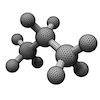
\includegraphics{images/logo.jpeg}\\
			To become the first logo for BU ProPANE.
			
		\subsection{Document Template}
			Decide to use \LaTeX as the default formatter for all formal documents. Decided on \LaTeX because it does the formatting and we want to focus on getting information on paper rather than formatting. \\
			\\
			The default template will start with a title page. The title page will include the title of the document as well as the names of the authors, the date it was created, and a summary of the contents of the document. The body of the document will be formatted using \LaTeX section, subsection, and subsubsection commands. 
			

\end{document}
